\section{Ejes de estudio}

Los ejes de estudio en los que nos centraremos son:
\begin{itemize}
    \item ¿Cómo varían las cancelaciones por clima a través del tiempo? ¿Cómo influye el aeropuerto de origen?
    \item ¿Cómo se comporta nuestro modelo de cuadrados mínimos con diferentes aerolineas? ¿Podemos predecir alguna mejor que otra?
\end{itemize}

\todo[inline]{REVISAR SI ES QUE REALMENTE HICIMOS ESTO QUE DICE}

En el primer eje trataremos de encontrar un patrón a las cancelaciones por clima a través del tiempo. ¿Se sigue un patrón regular?, ¿Hay fechas en las cuáles siempre hay cancelaciones? Veremos además que sucede con los retrasos en algunos aeropuertos particulares. \\

En el segundo eje analizaremos las aerolíneas. Nos centraremos en algunas más representativas y veremos las regularidades (o irregularidades) que poseen. ¿Hay alguna más dificil de predecir que otras? ¿Cómo se comporta una misma familia de funciones de cuadrados mínimos con distintas aerolineas? ¿Será necesario adaptarlo cada vez? \\

\section{Cancelaciones por clima}

\subsection{Preliminares}

En esta sección veremos cómo varían las cancelaciones por clima a través del tiempo, y veremos si podemos encontrar algún patrón. Nos será muy util contar con los motivos de las cancelaciones para poder diferenciar las que nos interesa, pero sin embargo, los datos previos a 2003 no cuentan con esta información. Es por eso que tomaremos los datos desde 2003 en adelante. \\

Con respecto a los gráficos que mostraremos, en un principio agrupamos los datos por mes pero con ello perdíamos información: hay valores que varían semana a semana dentro de un mismo mes. Por ello decidimos agrupar nuestros datos por semanas. \\

Sobre los retrasos, consideraremos que un vuelo tiene retraso cuando su tiempo de demora es superior a los 15 minutos. Esto se corresponde con la métrica de \textit{On Time Performance} (OTP) propuesta en el enunciado del trabajo. \\

\subsection{Experimentación}

En primer lugar tomaremos las cancelaciones por climas de manera general. Esperamos que haya una regularidad periódica, dónde para un mismo mes en diferentes años se registren cancelaciones comparables, pues tenemos en mente que hay épocas marcadas con tormentas fuertes o huracanes. \\

{\centering
    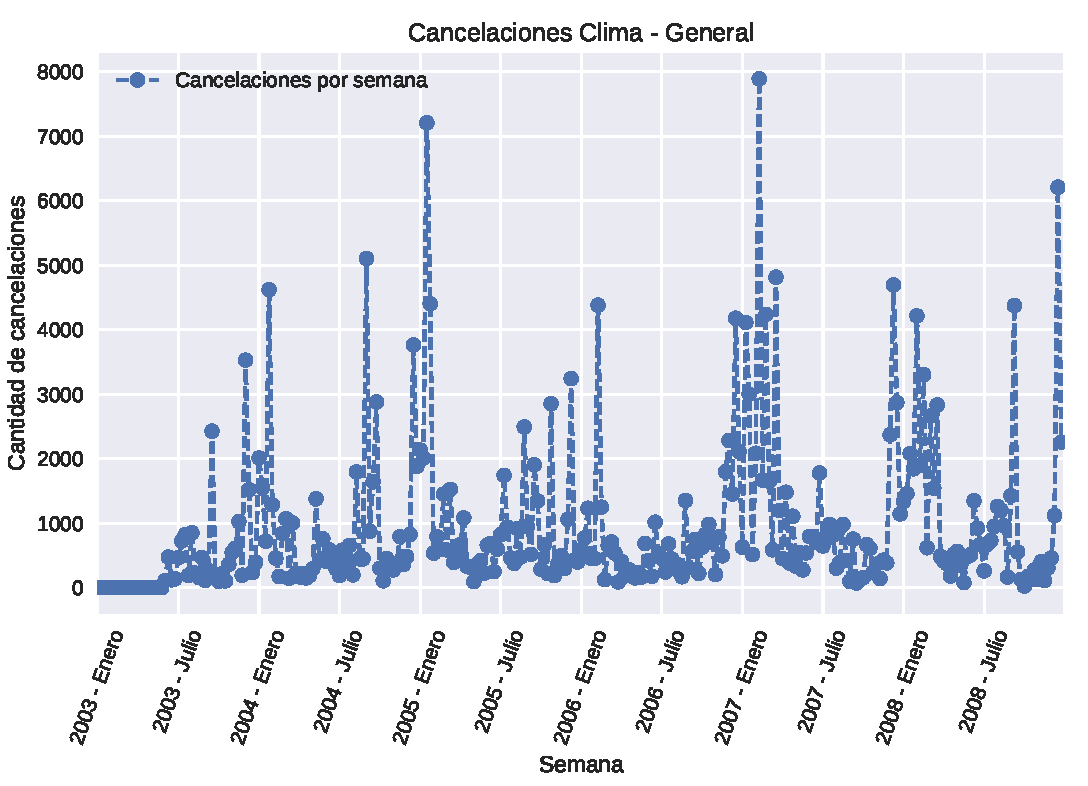
\includegraphics[scale=0.8]{informe/imagenes/cancelacionesClimaGeneralPlotV1.pdf} \\
    \captionof{figure}{Cancelaciones por clima con respecto al tiempo.\\}
}
$ $\newline

Analicemos un poco los datos. El comienzo de 2003 se ve completamente en cero, esto es por la falta de datos sobre cancelaciones climáticas en ese período. En las estimaciones de cuadrados mínimos no tendremos en cuenta este período sin datos, por lo que no nos será de ningún problema. \\

En enero y diciembre (invierno de USA) siempre se observan mayor cantidad de cancelaciones. Consideramos que esto puede deberse a dos motivos: Tormentas de nieve y mal clima en general, y el aumento del caudal de gente que viaja en épocas festivas. \\

En general, en agosto y septiembre se registran gran cantidad de cancelaciones, pero no es así todos los años. Por ejemplo, en 2007 no hay tanta cantidad como en 2004. Creemos que tiene que ver con las temporadas de huracanes, que no todos los años son catastróficas. Con respecto a nuestros datos, en agosto de 2004 el pico puede deberse al huracán Charley \cite{HuracanCharley}, mientras que agosto de 2005 se corresponde con el huracán Katrina \cite{HuracanKatrina}. \\

% @Jonno:  Esto se puede quitar, nomas me parecio piola como comentario
Como curiosidad, en agosto de 2003 se encuentra un pico aislado de los demás. Coincide con un apagón en grandes ciudades (Por ej, Nueva York) que duró 24hs en el cuál se reportaron cancelaciones de vuelos. Si bien uno creería que no tiene por qué estar relacionado al clima, el apagón se produjo por una caída del servicio central por las grandes demandas debido a las temperaturas inusuales de hasta 40 grados. \cite{ApagonNewYork} \\
% \subsection{Predicciones}

Para la predicción con cuadrados mínimos, la mejor familia de funciones que encontramos fue la siguiente:

\begin{align}
f(t) &= a + b * cos(\frac{\pi}{48} t)^{8} + c * sen(\frac{\pi}{24} t) + d * sen(\frac{\pi}{12} t)
\end{align}

Los períodos elegidos se corresponden con la cantidad de semanas. Por ejemplo, como sabemos que hay picos pronunciados en enero, tomamos $cos(\frac{\pi}{48} t)$ para que alcance un máximo cada 48 semanas. (En nuestros datos, cada mes está dividido en 4 semanas). La potencia a la cuál esta elevada fue elegida para que estos picos sean pronunciados en esas fechas. Análogamente con los períodos de los senos, queremos que se tengan en cuenta los ciclos de seis meses y tres meses respectivamente. \\

{\centering
    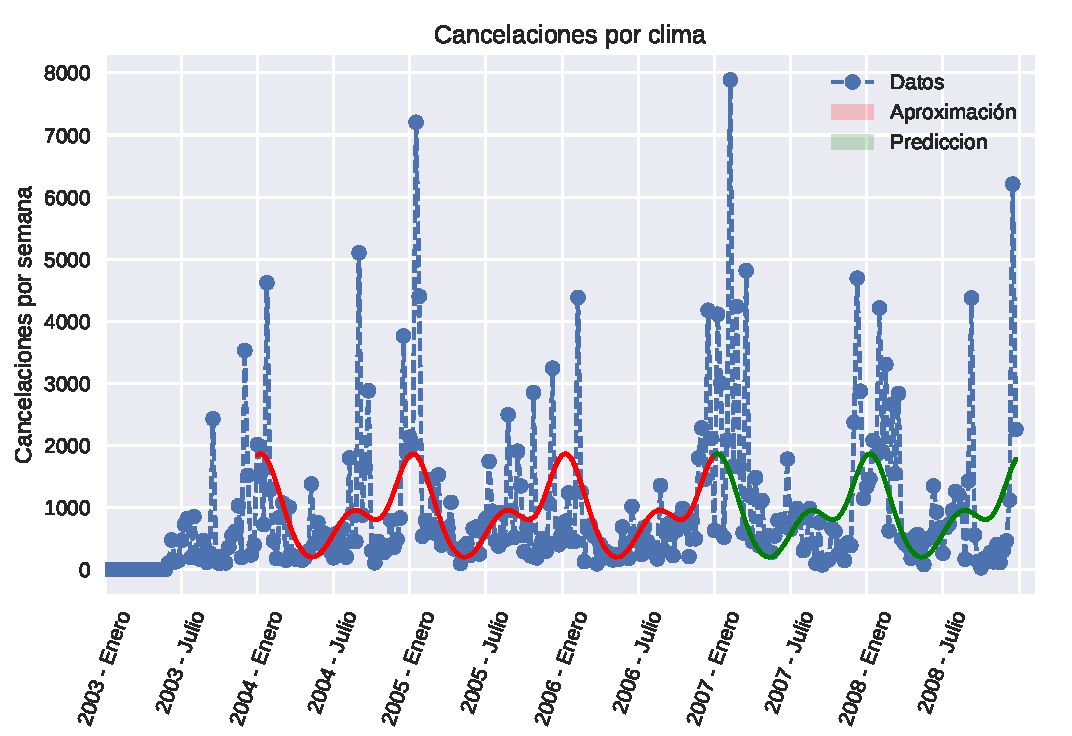
\includegraphics[scale=0.8]{informe/imagenes/cancelacionesPorClimaGeneralPrediccionV1.pdf} \\
    \captionof{figure}{Cancelaciones por clima, 3 años de entrenamiento y 2 de predicción.\\}
}

% @Jonno, con periodos de 2 años de train y 1 de prediccion:
% ECM: 1130960.72329
% ECM: 1991041.60249
% ECM: 671208.89326
Con esta familia de funciones obtuvimos (promediando con Cross Validation) un ECM de 1264403. Las cancelaciones por clima en general no fueron sencillas de predecir, y no obtuvimos resultados muy buenos. Diferentes aeropuertos podrían estar sumando cancelaciones en períodos diferentes, es por esto que en el siguiente experimento mostramos dos aeropuertos particulares: los aeropuertos de Miami y Los Ángeles. La razón de la elección es porque ambos se encuentran en costas opuestas del país, y porque Miami suele sufrir cancelaciones por mal clima sobre todo en época de huracanes (Agosto). \\

Una aclaración importante: en los datos de Miami quitamos dos valores outliers que representaban mas de 450 cancelaciones esa semana pues distorsionaban el gráfico completamente. Creemos que correspondían al huracán Charley y Katrina. De todos modos, sus respectivos picos en esas fechas se siguieron manteniendo. \\

Para ambos aeropuertos consideraremos la misma familia de funciones que en el experimento anterior, y realizamos Cross Validation para medir los errores. Para Miami obtubimos un ECM de 227. Con Los Ángeles, el ECM fue de 180.

% @Jonno - Miami
% ECM: 442.585074873
% ECM: 194.785193426
% ECM: 45.2682310293

% @Jonno - Los Angeles
% ECM: 169.919233204
% ECM: 254.398202871
% ECM: 119.879984961


\begin{figure}[H]
\centering
\begin{minipage}{.5\textwidth}
  \centering
  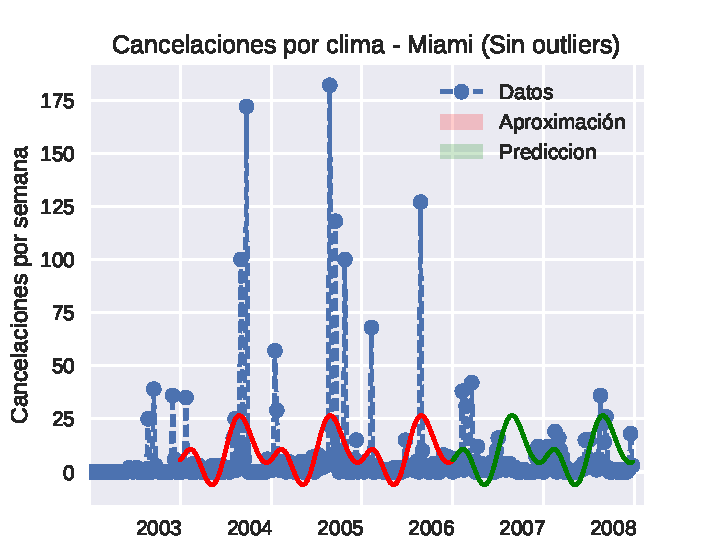
\includegraphics[width=1.1\linewidth]{informe/imagenes/cancelacionesClimaMiamiPrediccionV1.pdf}
  \captionof{figure}{Clima - Miami}
\end{minipage}%
\begin{minipage}{.5\textwidth}
  \centering
    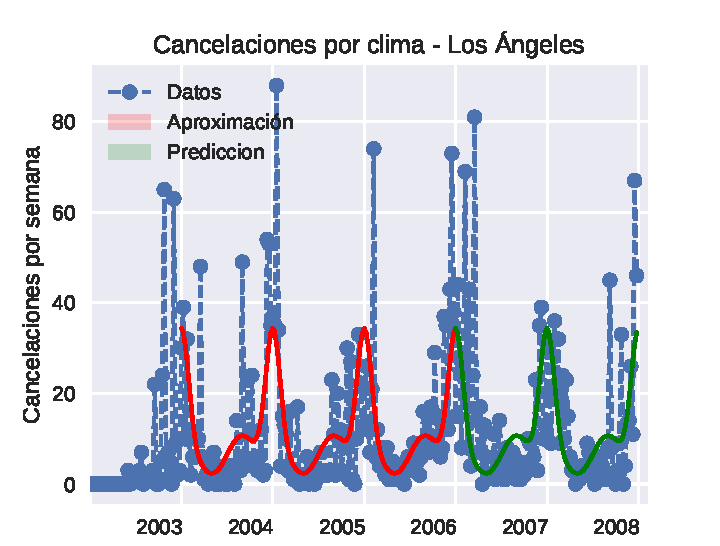
\includegraphics[width=1.1\linewidth]{informe/imagenes/cancelacionesClimaLosAngelesPrediccionV1.pdf}
    \captionof{figure}{Clima - Los Ángeles}
\end{minipage}
\end{figure}

Diferentes aeropuertos tienen diferentes cantidades de cancelaciones, sin embargo en los aeropuertos en los que experimentamos encontramos resultados similares, incluso en los que no mostramos. En los meses de diciembre y enero podemos siempre encontrar los mayores picos de cancelaciones por clima. Además, en los meses de julio y agosto también suelen registrarse picos (aunque de menor altura). \\

En conclusión, gracias a la periodicidad anual y semestral de las cancelaciones por clima, la familia de funciones que fijamos al comienzo de la sección sirve como un buen predictor para distintos aeropuertos. \\

\section{Aerolíneas}
